\documentclass[a4paper,12pt]{article}


% --------------------------------------------------------------------------- %
\usepackage{graphicx}

\usepackage[utf8]{inputenc}             % Encodamento utf-8
\usepackage[brazil]{babel}              % Parcote para texto em português

\usepackage{setspace}                   % Espaçamento flexível
\usepackage{indentfirst}                % Indentação do primeiro parágrafo
\usepackage[fixlanguage]{babelbib}      % Opções extras para linguagem

\usepackage[usenames,svgnames,dvipsnames]{xcolor}
\usepackage[font=small,format=plain,labelfont=bf,up,textfont=it,up]{caption}
\usepackage[a4paper,top=2.54cm,bottom=2.0cm,left=2.0cm,right=2.54cm]{geometry}

\usepackage[pdftex,plainpages=false,pdfpagelabels,pagebackref,colorlinks=true,citecolor=DarkGreen,linkcolor=NavyBlue,urlcolor=DarkCornflowerBlue,filecolor=green,bookmarksopen=true]{hyperref} 				% links coloridos
\usepackage[all]{hypcap}                % soluciona o problema com o hyperref 
					% e capitulos

\newpage %%%%%%%%%%%%%%%%%%%%%%%%%%%%%%%%%%%%%%%%%%%%%%%%%%%%%%%%%%%%%%%%%%%%%%
  \pagenumbering{arabic}     % começamos a numerar 
  \begin{document}

  \begin{center}
	{\LARGE \textcolor{NavyBlue}{ \textbf{Manual de usuário - Jogo das Canoas}}}
  \end{center}

  \bigskip
  \bigskip

  O Jogo das Canoas consiste, nessa fase, em gerar um rio com 
  características atribuídas pelo próprio usuário, sendo essas características 
  frequência, probabilidade e tamanho das ilhas e largura, altura e distância
  mínima entre as margens do rio. O rio que será gerado de acordo com as 
  características atribuídas pelo usuário, é gerado em 
  interface gráfica com cores e uma canoa que não tem movimentos.


\newpage %%%%%%%%%%%%%%%%%%%%%%%%%%%%%%%%%%%%%%%%%%%%%%%%%%%%%%%%%%%%%%%%%%%%%%
\section{\textcolor{NavyBlue}{Compilação}}

Para compilar o jogo, entre na pasta onde o seu jogo se localiza e utilize o seguinte comando no terminal:

\$ \textcolor{CornflowerBlue}{\textit{make}}

\bigskip
\section{\textcolor{NavyBlue}{Execução}}

  Para inicializar o jogo, após compilá-lo, digite no próprio terminal:
  
  \$ \textcolor{CornflowerBlue}{\textit{./bin/ep2}}
  
  Digitando esse comando, irá aparecer o seguinte:


  \begin{verbatim}
  ........................   .........................................
  :::::::::::::::::::::::::.   '::::::::::::::::::::::::::::::::::::::
  ;;;;;;;;;;;;;;;;;;;;;;;;;;;.      ::;;;;;;;;;;;;;;;;;;;;;;;;;;;;;;;;
  +++++++++++++++++++++++++++++        +++++++++++++++++++++++++++++++
  +++++++++++++++++++++++++++++++         ++++++++++++++++++++++++++++
  ++++++++++++++++++++++++++++++++           +++++++++++++++++++++++++
  ================================             =======================
  ===============================                =====================
  oooooooooooooooooooooooooooooo                   ooooooooooooooooooo
  oooooooooooooooooooooooooooo                      oooooooooooooooooo
  $$$$$$$$$$$$$$$$$$$$$$$$$    ,   .                 $$$$$$$$$$$$$$$$$
  $$$$$$$$$$$$$$$$$$$$$$$    ,','''''.'''            $$$$$$$$$$$$$$$$$
  $$$$$$$$$$$$$$$$$$$$     ,'Y|______Y'.|            $$$$$$$$$$$$$$$$$
  ##################    _,',|______,'   '.          ##################
  ###############      | ,'      ,'   ,'  |'|      ###################
  #############        ,'______,'   ,'    |_|    #####################
  @@@@@@@@@@           \       /  ,'           @@@@@@@@@@@@@@@@@@@@@@@
  @@@@@@@               \     / ,'           @@@@@@@@@@@@@@@@@@@@@@@@@
  @@@@                   '---'             @@@@@@@@@@@@@@@@@@@@@@@@@@@

  --------------------------------------------------------------------
                          JOGO DAS CANOAS!                            
  --------------------------------------------------------------------
                                                                      
   1) Jogar                                                           
   2) Configurar jogo                                                 
   3) Modo teste (simples)
   4) Modo teste (completo)
   5) Sair
  
  \end{verbatim}

\newpage %%%%%%%%%%%%%%%%%%%%%%%%%%%%%%%%%%%%%%%%%%%%%%%%%%%%%%%%%%%%%%%%%%%%%%%%%%%%%%%%%%

  Depois, basta digitar o que se deseja fazer no terminal,
  de acordo com o menu acima.
  
  \bigskip

  \textcolor{CornflowerBlue}{1} inicializa o jogo em modo interface gráfica.
  
  \textcolor{CornflowerBlue}{2} pergunta se você deseja modificar determinada 
  configuração,
  em caso afirmativo ele pede para que o valor seja inserido.
  
  \textcolor{CornflowerBlue}{3} dá as informações de última linha de um 
  determinado frame.
  
  \textcolor{CornflowerBlue}{4} dá as informações de todas as linhas de um 
  determinado frame.
  
  \textcolor{CornflowerBlue}{5} finaliza o programa.
  
  \bigskip  

  Quando a resposta a uma pergunta for afirmativa (yes/sim), basta digitar no 
  terminal, 's', 'y', 'S' ou 'Y'.
  
  Porém, quando a resposta for negativa, basta digitar no terminal 'n' ou 'N'.
  \bigskip
  \bigskip  

  Por exemplo:
  
  Pergunta: "\textcolor{NavyBlue}{Deseja configurar o fluxo do rio? }"
  
  Se sim:   '\textcolor{NavyBlue}{s}', '\textcolor{NavyBlue}{y}',
  '\textcolor{NavyBlue}{S}' ou '\textcolor{NavyBlue}{Y}'
  
  Se não:   '\textcolor{NavyBlue}{n}' ou '\textcolor{NavyBlue}{N}'


\newpage %%%%%%%%%%%%%%%%%%%%%%%%%%%%%%%%%%%%%%%%%%%%%%%%%%%%%%%%%%%%%%%%%%%%%%%


  \bigskip
  \subsection{\textcolor{NavyBlue}{Características adicionais}}
  
  Também é possível adicionar as características através de comandos no terminal 
  quando o arquivo é executado:
  
  Basta digitar colocar o comando de execução + a característica que se deseja 
  modificar + seu novo valor. Tudo isso fica mais claro nos exemplos abaixo.
  
  \bigskip
  \begin{itemize}
  
  \item Fluxo do rio . . . . . . . . . . . . . . . . . . .  \textcolor{CornflowerBlue}{-F}
  \item Altura do rio. . . . . . . . . . . . . . . . . . .  \textcolor{CornflowerBlue}{-H}
  \item Largura do rio . . . . . . . . . . . . . . . . . .  \textcolor{CornflowerBlue}{-L}
  \item Frequência das ilhas . . . . . . . . . . . . . . .  \textcolor{CornflowerBlue}{-i} 
  \item Distância de segurança entre ilhas. . . . . . .  \textcolor{CornflowerBlue}{-f}
  \item Semente geradora de aleatoriedade . . . . . .  \textcolor{CornflowerBlue}{-s}
  
  \end{itemize}
  \bigskip
  
  Caso você queira ver o programa rodando em modo teste, num número fixo de
  iterações, existem também as seguintes opções disponíveis:
  
  \bigskip
  \begin{itemize}
  
  \item Teste simples  . . . . . . . . . . . . . . . . . . .   \textcolor{CornflowerBlue}{-t}
  \item Teste completo . . . . . . . . . . . . . . . . . .  \textcolor{CornflowerBlue}{-T}
  \item Número de iterações  . . . . . . . . . . . . . . .  \textcolor{CornflowerBlue}{-N}
  \item Arquivo de saída para os testes  . . . . . . . . .  \textcolor{CornflowerBlue}{-o} 
  
  \end{itemize}
  \bigskip
  
  O teste simples imprime um relatório sobre o último frame gerado,
  enquanto o teste completo mostra dados sobre o rio linha a linha. 
  O arquivo de saída deve conter, no máximo, 20 caracteres (incluin-
  do a extensão.
  
  \bigskip
  \bigskip
  \bigskip
  
  Observação: Existe uma opção adicional \textcolor{CornflowerBlue}{-h}, 
  caso você precise de ajuda.
  
  \newpage %%%%%%%%%%%%%%%%%%%%%%%%%%%%%%%%%%%%%%%%%%%%%%%%%%%%%%%%%%%%%%%%%%%%
  \subsection{\textcolor{NavyBlue}{Exemplos de utilização:}}
  \bigskip
  
    \subsubsection{\textcolor{NavyBlue}{Exemplo 1}}
    \bigskip
    \begin{itemize}
  
    \item Altura do rio = 30  . . \textcolor{CornflowerBlue}{-H30}
    \item Largura do rio = 60  . . \textcolor{CornflowerBlue}{-L60}  
    \item Distância mínima entre as margens = 35  . . \textcolor{CornflowerBlue}{-Z20}
    
    \end{itemize}  
    \bigskip
    
    \$ \textcolor{CornflowerBlue}{\textit{make}}
    
    \$ \textcolor{CornflowerBlue}{\textit{./bin/ep2 -H30 -L60 -Z20}}
  
    \bigskip
    
\begin{figure}[h]
     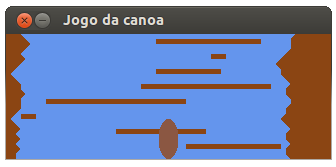
\includegraphics[scale=1]{im1.png}
     \caption{Legenda da Imagem}
\end{figure}
  
  \newpage %%%%%%%%%%%%%%%%%%%%%%%%%%%%%%%%%%%%%%%%%%%%%%%%%%%%%%%%%%%%%%%%%%%%
    \subsubsection{\textcolor{NavyBlue}{Exemplo 2}}
    
    \begin{itemize}
    \bigskip
    
    \item Fluxo do rio = 20  . . \textcolor{CornflowerBlue}{-F20}  
    \item Altura do rio = 25  . . \textcolor{CornflowerBlue}{-H25}
    \item Largura do rio = 65  . . \textcolor{CornflowerBlue}{-L65}
    \item Frequência das ilhas = 80\%  . . \textcolor{CornflowerBlue}{-i0.8}
    \item Distância mínima entre ilhas = 2  . . \textcolor{CornflowerBlue}{-f2}
    \item Semente geradora de aleatoriedade = 10  . . \textcolor{CornflowerBlue}{-s10}
    \item Distância mínima entre as margens = 35  . . \textcolor{CornflowerBlue}{-Z35}
    
    \end{itemize}  
    \bigskip
    
    \$ \textcolor{CornflowerBlue}{\textit{make}}
    
    \$ \textcolor{CornflowerBlue}{\textit{./bin/ep2 -F20 -H25 -L65 -i0.8 -f2 -s10 -Z35}}
    
    \bigskip

  \begin{figure}[h]
     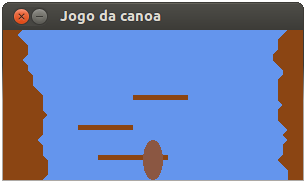
\includegraphics[scale=1]{im2.png}
     \caption{Legenda da Imagem}
\end{figure}

\end{document}
